 %!TeX root = Chapter_SignalAnalysis
\documentclass[../../CompleteThesis/Complete_1stDraft]{subfiles}

\begin{document}
	The data obtained through various experimental measurements are easily compared with a time series, as they typically show some quantity measured all along the depth of an ice core. This depth is often, at short intervals, treated as a regular linear time series thus making it possible to use some of the known signal analysis methods. Of course, when considering the entirety of an ice core, the linearity disappears as thinning and compression makes the depth series non linear. But when considering short lengths of core it is possible to estimate a linearity, assuming conformity in this specific layer. 
	
	\section[Synthetic Data]{Diffusion Illustrated through Synthetic Data}
	\label{Sec:SignalAnalysis_SyntheticData}
	\todo{SIGNAL-SYNTHDATA: Write about synthetic data generation.}
	
	\begin{figure}[h]
		\centering
		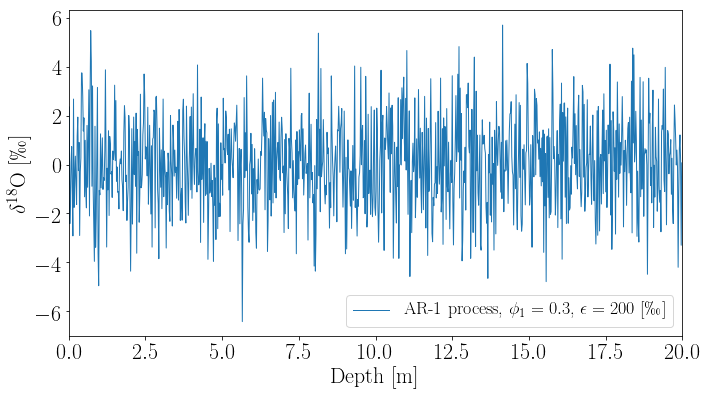
\includegraphics[width=0.8\textwidth]{AR1_process.png}
		\caption[]{}
		\label{fig:AR1_process}
	\end{figure}
	
	\begin{figure}[h]
		\centering
		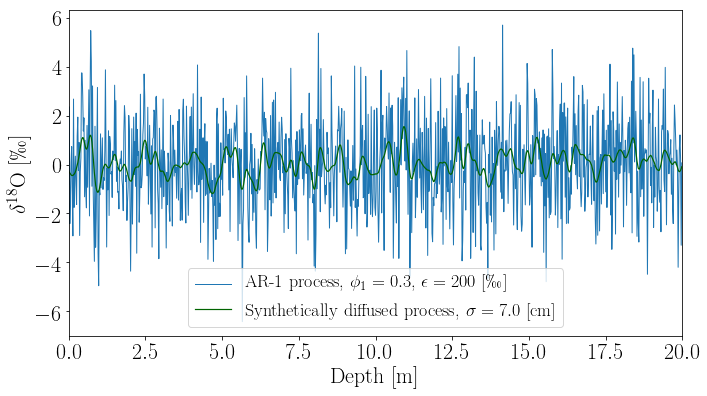
\includegraphics[width=0.8\textwidth]{AR1_process_W_backDiff.png}
		\caption[]{}
		\label{fig:AR1_process_W_backDiff}
	\end{figure}
	
	\begin{figure}[h]
		\centering
		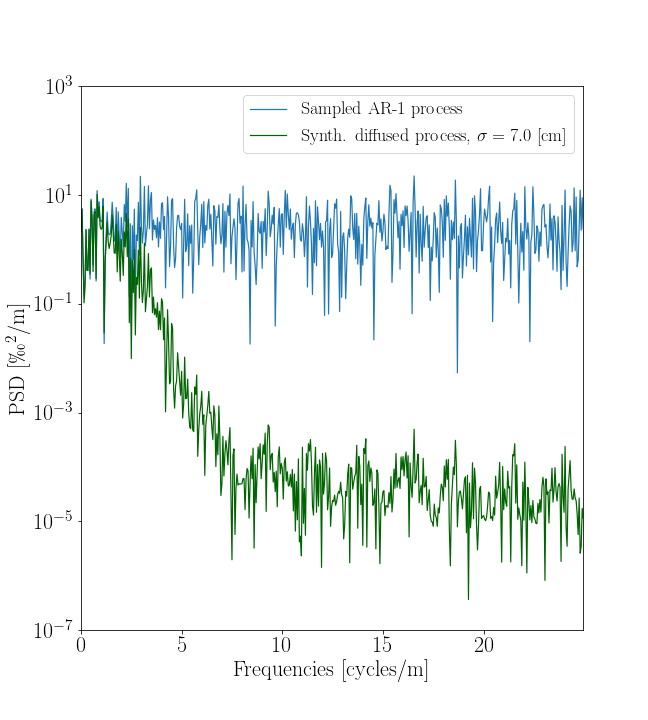
\includegraphics[width=0.6\textwidth]{AR1_process_W_backDiff_PSD.png}
		\caption[]{}
		\label{fig:AR1_process_W_backDiff_PSD}
	\end{figure}
	
	
	
	
	
	
	
	
	\section[Back Diffusion][Back Diffusion]{Back Diffusion}
	\label{Sec:SignalAnalysis_BackDiffusion}
	Due to diffusion in firn and ice, some of the water isotopic signal is lost. Some of this signal can be restored by investigating the diffusion process, and through filtering and deconvolution techniques(REFERENCES).
	For the data of this thesis two different restoration techniques are presented: a spectral method, determining the effect of mixing and diffusion as a spectral filter(REFERENCES), and a kernel restoration method much like the ones used to restore pixel resolution in images (REFERENCES). 
	\subsection[Spectral Analysis][Spectral Analysis]{Spectral Analysis}
	\label{Subsec:SignalAnalysis_BackDiffusion_SpectralAnalysis}
	\subsubsection[PSD][PSD]{Power Spectral Densities}
	\label{Subsubsec:SignalAnalysis_BackDiffusion_SpectralAnalysis_PSD}
	A very useful tool for analyzing signals exhibiting oscillatory effects is analysis of the signals power spectrum. Instead of considering the signal in time, it is transformed to the spectral domain, where it is possible to obtain an estimate of both the signal and the underlying noise. This is crucial for enhancing the signal and filtering away noise. But to be able to examine these effects, first the data must be transformed. A range of different methods may be used to compute the frequency transform of the depth series, here I present the three I have been working with. Since the data are discrete and experimental, I will be presenting the discrete and applicable mathematical models.\\
	When considering a signal, it may be of interest to investigate how the energy of said signal is distributed with frequency. The total power is defined as:
	\begin{equation}
		\text{Total Power} = \int_{-\infty}^{\infty} |X(\tau)|^2 \, d\tau.
		\label{Eq:SignalEnergy}
	\end{equation}
	Using Parseval's theorem (REFERENCE) (assuming that the signal has a finite total energy), the power of the signal can alternatively be written as
	
	\begin{equation}
		\int_{-\infty}^{\infty} |X(\tau)|^2 \, d\tau = \int_{-\infty}^{\infty} |\tilde{X}(\tau)|^2\, df
		\label{Eq:ParsevalsTheorem}
	\end{equation}
	where $\tilde{X}(f)$ is the spectral (Fourier) transform of the signal, from time to frequency domain, defined as:
	\begin{equation}
		\tilde{X}(f) = \int_{-\infty}^{\infty} X(\tau) e^{2\pi i f \tau} \, d\tau
		\label{Eq:FourierTransform}
	\end{equation}
	and the inverse spectral (Fourier) transform, from frequency to time domain, defined as:
	\begin{equation}
		X(t) = \int_{-\infty}^{\infty} \tilde{X}(f) e^{-2\pi i f \tau}\, df.
		\label{Eq:InverseFourierTransform}
	\end{equation}
	Both $X(t)$ and $\tilde{X}(f)$ represent the same function, just in different variable domains. Often, the angular frequency $\omega$ is used instead, with the relation between $\omega$ and $f$ being $\omega \equiv 2\pi f $, giving the Fourier and inverse Fourier transforms as:
	
	\begin{equation}
		\begin{aligned}
			\tilde{X}(\omega) &= \int_{-\infty}^{\infty} X(t) e^{i\omega\tau}\, d\tau \\
			X(\tau) &= \int_{-\infty}^{\infty} \tilde{X}(\omega) e^{-i\omega\tau}\, d\omega
			\label{Eq:FourierTransformAngular}
		\end{aligned} 
	\end{equation}
	
	From Equation \ref{Eq:ParsevalsTheorem} we can interpret the integrand on the right hand side $|\tilde{X}(f)|^2$ as a density function, describing the energy per unit frequency. This is a property which is able to reveal much information about the considered signal, and it is useful to define this as the (one-sided) Power Spectral Density: 
	\begin{equation}
		P_X(f) \equiv |\tilde{X}(f)|^2 + |\tilde{X}(-f)|^2 \qquad 0 \leq f < \infty
	\end{equation}
	This entity ensures that the total power is found just by integrating over $P_X(f)$ from 0 to $\infty$. When the function is purely real, the PSD reduces to $P_X(f) = 2|\tilde{X}(f)|^2$.\\
	In the above the transform used to define the PSD was presented as the Fourier transform. When working with discrete data, as is very common when analyzing real world data, there are a number of different ways of estimating the PSD. In the following three different methods will be presented, all used in this thesis.
	\newline
	\todo{SIGNAL-BACKDIFF: RETHINK THIS PART. DO NOT USE TIME ON ALL THE CALCULATIONS. WRITE THE GENERAL IDEAS OF THE METHODS AND STATE HOW TO CALCULATE/COMPUTE. SMALL CODE SNIP TO GIVE GENERAL IDEA.}
	\begin{quote}
		\textcolor{red}{\textbf{RETHINK THIS PART. DO NOT USE TIME ON ALL THE CALCULATIONS. WRITE THE GENERAL IDEAS OF THE METHODS AND STATE HOW TO CALCULATE/COMPUTE. SMALL CODE SNIP TO GIVE GENERAL IDEA.}}
	\end{quote}


	\subsubsection[Spectral Transforms][Spectral Transforms]{Spectral Transforms}
	\label{Subsubsec:SignalAnalysis_BackDiffusion_SpectralAnalysis_SpectralTransforms}
	
	\begin{itemize}
		\item DFT/FFT
		\item NUDFT
		\item DCT
		\item NDCT
		\item (MEM)
	\end{itemize}


	\begin{figure}[h]
		\centering
		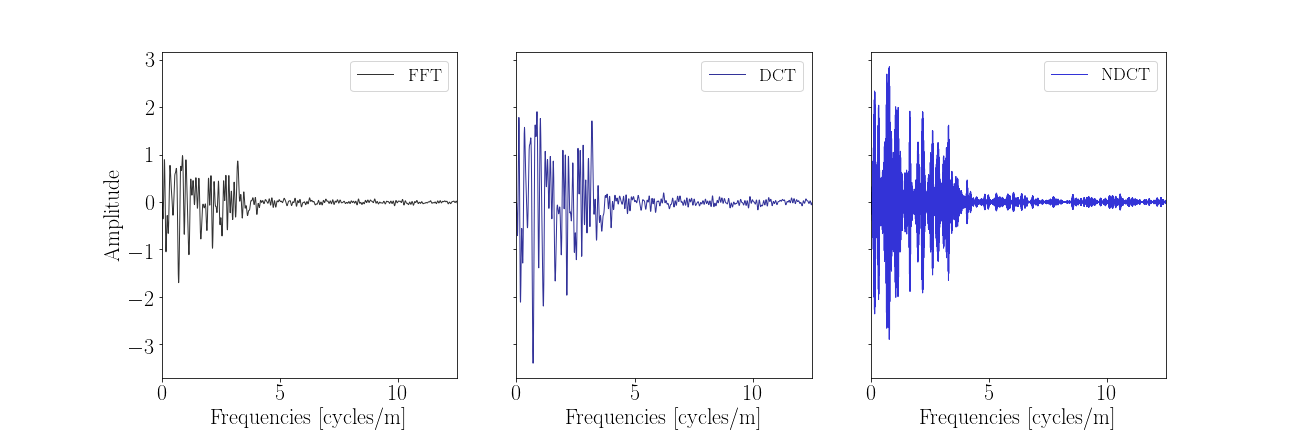
\includegraphics[width=\textwidth]{SpectralTransforms_3.png}
		\caption[FFT, DCT, NDCT, Site A]{Examples of three different spectral transforms, FFT, DCT, NDCT, performed on the depth series between Tambora and Laki eruptions from Site A.}
		\label{fig:SpectralTransforms_3}
	\end{figure}
	
	\begin{figure}[h]
		\centering
		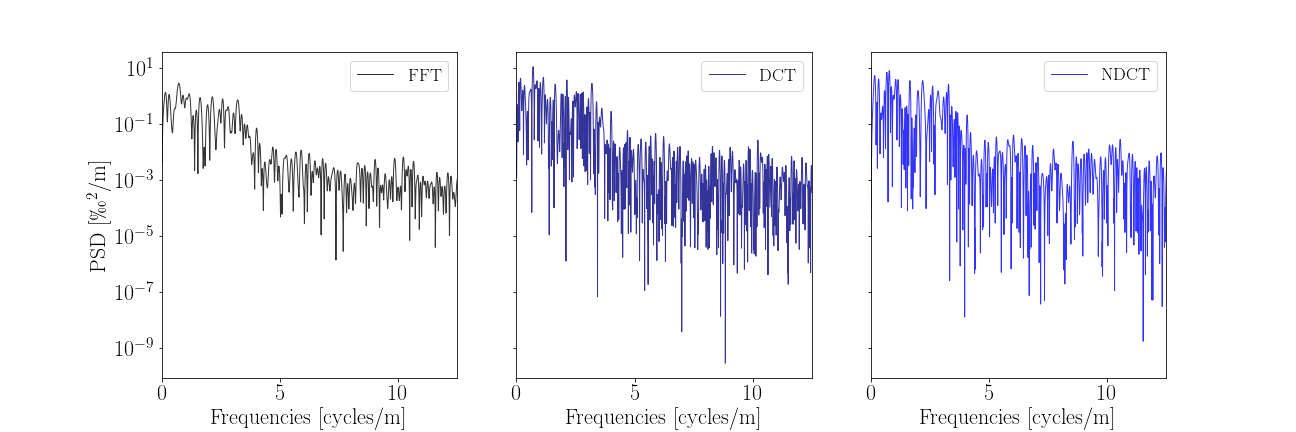
\includegraphics[width=\textwidth]{SpectralTransforms_PSD.png}
		\caption[FFT, DCT, NDCT PSDs, Site A]{Examples of power spectral densities related to the three different spectral transforms, FFT, DCT, NDCT, seen in Figure \ref{fig:SpectralTransforms_3}.}
		\label{fig:SpectralTransforms_PSD}
	\end{figure}
	
	
	
	\subsection[Spectral Filtering][Spectral Filtering]{Spectral Filtering}
	\label{Subsec:SignalAnalysis_BackDiffusion_SpectralFiltering}
	\subsubsection[Wiener Filtering][Wiener Filtering]{Wiener Filtering}
	\label{Subsubsec:SignalAnalysis_BackDiffusion_SpectralFiltering_Wiener}
	Through spectral analysis it is possible to treat the noise of the signal consistently. The goal is to create spectral filters which enhances the signal while minimizing the effect of the noise, thus increasing the signal-to-noise ratio (SNR).\\
	Theoretically, without any diffusion, the change in isotopic concentration would be described through a step function, going from one constant concentration to another. This step function can be described by the Heaviside function:
	\begin{equation}
		D(t) = \begin{cases}
			0, & t < 0 \\
			1, & t \geq
		\end{cases}
	\end{equation}
	In reality, a number of different mixing processes change this step function, and the measured signal will be a smooth curve, $s(t)$, which corresponds to the convolution of $S(t)$ with the mixing response function $M(\tau)$
	\begin{equation}
		d(t) = \int_{- \infty}^{\infty} D(\tau) \cdot M(t - \tau)d\tau
	\end{equation}
	
	
	\subsection[Signal Restoration][Signal Restoration]{Signal Restoration by Optimal Diffusion Length}
	\label{Subsec:SignalAnalysis_BackDiffusion_SignalRestoration}
	\subsubsection{Kernel Estimation}
	\label{Subsubsec:SignalAnalysis_BackDiffusion_SignalRestoration_KernelEstimation}
	As is well known, in the spectral domain, convolution is multiplication and the mixing is described as the multiplication between the Fourier transform of $S$ and $M$:
	\begin{equation}
		\tilde{d} = \tilde{D} \cdot \tilde{M}
	\end{equation}
	
	
	By differentiation with respect to time, the mixing filter $M$ is unaffected, and differentiation of the measured system response, the Heaviside function, $S'$ is a delta function, which Fourier transformed is unity, leading to:
	\begin{equation}
		\tilde{d'} = \tilde{D'} \cdot \tilde{M} = \tilde{M}
	\end{equation}
	The mixing filter can thus be determined by measuring the system response to a step function, differentiating performing Fourier transform of the result $d'$.
	
	After determination of the mixing filter $\tilde{M}$, the unmixed signal $D$ can be estimated in theory by inverse Fourier transform of
	
	
	\begin{equation}
		\tilde{D} = \tilde{d}\cdot\tilde{M}^{-1}
		\label{eq:Restoration}
	\end{equation}
	
	During the mixing, cycles with short wavelengths are heavily washed out, and through the restoration in Eq. \ref{eq:Restoration}, the amplitudes corresponding to these wavelengths are heavily amplified by the filter. This method though has a drawback, which is that when the measurements contain noise, the restored signal will be dominated by high-frequency noise, greatly amplified by the mixing filter. Thus it is a problem of retaining as much (short wavelength) signal as possible while simultaneously attempting to amplify the high-frequency noise as little as possible. This optimal trade-off can be found by creating an optimum filter for the considered measured isotopic signal:
	\begin{equation}
		\delta_M(z) = \delta_m (z) + \eta(z)
	\end{equation} 
	This optimal (Wiener) filter $\tilde{F}$, defined for each wave number $k = 2\pi \omega$, is presented as the ratio between pure signal and pure signal plus noise described in Power Spectral Densities as:
	\begin{equation}
		\tilde{F}(k) =\frac{|\tilde{\delta_m}(\omega)|^2}{|\tilde{\delta_m}(\omega)|^2 + |\tilde{\eta}(\omega)|^2}
		\label{eq:WienerFilter}
	\end{equation}
	In this work, the power spectral densities of the signal and the noise, respectively, are determined through analysis of the power spectral density of the combined signal/noise PSD.\\
	The PSD of the noise free measured signal, $|\tilde{\delta_m}(\omega)|^2$, is assumed describe as 
	\begin{equation}
		|\tilde{\delta}_m(\omega)|^2 = P_0 e^{-k^2 \sigma_{\text{tot}}^2}
		\label{eq:SignalPSD}
	\end{equation}
	where $\sigma_{\text{tot}}^2$ describes the total estimated diffusion length of the mixing.\\
	The noise is assumed to be red noise, described by an autoregressive process of first order, AR1:
	\begin{equation}
		|\tilde{\eta}(\omega)|^2 = \frac{\sigma_{\eta}^2 \Delta z}{|1 + a_1 \exp(-2\pi i \omega \Delta z)|^2}
		\label{eq:NoisePSD}
	\end{equation}
	where $\sigma_{\eta}^2$ is the variance of the red noise, $a_1$ is the AR1 coefficient and $\Delta z$ is the resolution of the time/depth data.
	It is then possible to estimate the parameters $P_0$, $\sigma_{\text{tot}}^2$, $\sigma_{\eta}^2$ and $a_1$ by curve fitting, separately, the two expressions in Eq. \ref{eq:SignalPSD} and \ref{eq:NoisePSD} to the data. The estimated parameters are varied to find the optimal guess to use for the filter.
	
	\begin{figure}
		\centering
		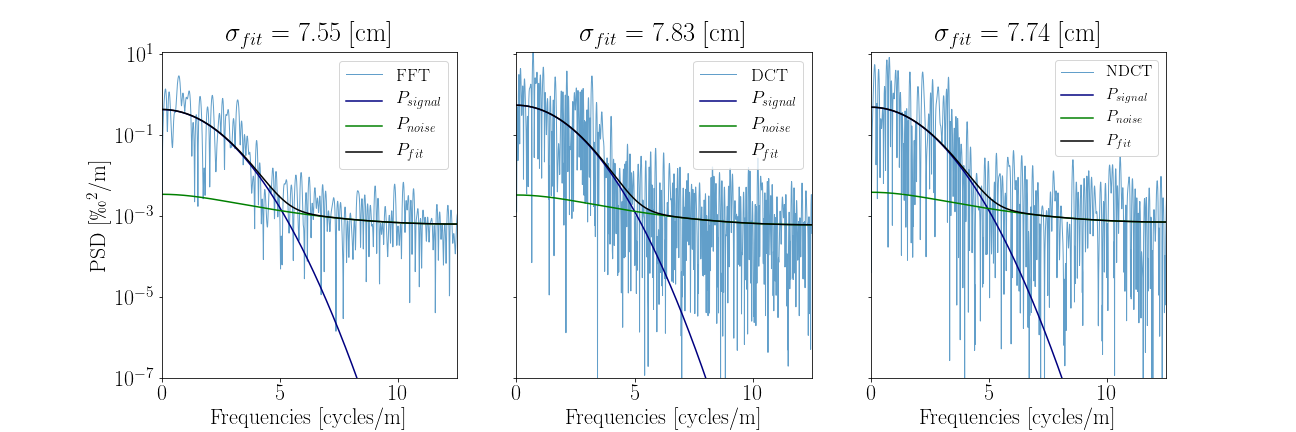
\includegraphics[width=\textwidth]{SpectralTransforms_PSDwFits.png}
		\caption[FFT, DCT, NDCT PSDs with Fit, Site A]{Noise, signal and total fit to PSD, illustrating the construction of the Wiener Filter, see Sec. \ref{Sec:SignalAnalysis_Restoration}.}
		\label{fig:SpectralTransforms_PSDwFits}
	\end{figure}
	
	
	\section[Restoration][Restoration]{Enhanced Resolution and Restoration of Signal}
	\label{Sec:SignalAnalysis_Restoration}
	
	\subsection[Interpolation]{Interpolation of Data}
	\label{Subsec:SignalAnalysis_Restoration_Interpolation}
	For the purpose of this thesis, interpolation of data needs to be fast, efficient and result in a function as smooth as possible. The last criterion is due to the knowledge of the nature of the data. The measurements are not continuous but should indeed in theory be so. Thus a good choice for interpolation of the data examined in this thesis would be the cubic spline interpolation. An instance of a such interpolation can be seen in Figure \ref{fig:Interp}.\\
	Cubic spline interpolation has been used in two instances during this analysis, both times through the \lstinline[language=Python]|Python SciPy| package \lstinline[language=Python]|scipy.interpolate.CubicSpline|\todo{SIGNAL-INTERP: REFERENCE!!}. Firstly, to assure equally spaced data points, so as to be able to perform a useful frequency analysis through spectral transformation, see Section, \ref{sec:???}. Secondly cubic spline interpolation was used to improve on peak detection in the final back diffused data. The final data have a rather low resolution, leading to an initial guess of peak positioning that might be shifted due to the discretization. Through cubic spline interpolation it is possible to construct a smooth estimate of a signal of higher resolution, leading to a peak positioning estimate that might be less shifted, see Figure \ref{fig:InterpFinal}.
	
	\subsection[Standardisation]{Detrending and Standardising}
	\label{Subsec:SignalAnalysis_Restoration_Standardisation}
	
	\todo{SIGNAL-STANDARD: Think about if this is necessary. Maybe work into recursivity and constraints in Method?}
	\subsection[Cycle Length Estimation][Cycle Length Estimation]{Cycle Length Estimation of Detrended Signal}
	\label{Subsec:SignalAnalysis_Restoration_CycleLengthEst}
	\todo{SIGNAL-CYCLE: Think about if this is necessary. Maybe work into recursivity and constraints in Method?}
	
\end{document}
